

\tikzset{every picture/.style={line width=0.75pt}} %set default line width to 0.75pt        

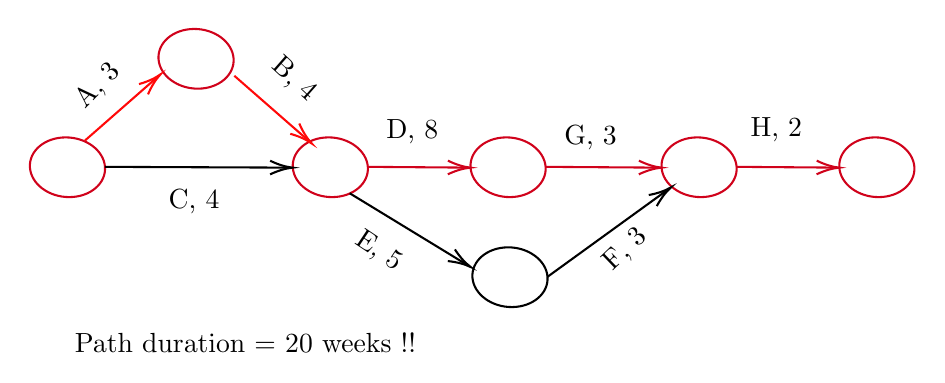
\begin{tikzpicture}[x=0.75pt,y=0.75pt,yscale=-1,xscale=1]
%uncomment if require: \path (0,167); %set diagram left start at 0, and has height of 167

%Shape: Ellipse [id:dp3231871162362072] 
\draw  [color={rgb, 255:red, 208; green, 2; blue, 27 }  ,draw opacity=1 ] (46.99,75.24) .. controls (47.58,83.19) and (39.98,89.72) .. (29.99,89.82) .. controls (20.01,89.93) and (11.43,83.58) .. (10.83,75.63) .. controls (10.24,67.68) and (17.84,61.15) .. (27.83,61.05) .. controls (37.81,60.94) and (46.39,67.3) .. (46.99,75.24) -- cycle ;
%Shape: Ellipse [id:dp6149438789896213] 
\draw  [color={rgb, 255:red, 208; green, 2; blue, 27 }  ,draw opacity=1 ] (108.94,22.99) .. controls (109.54,30.94) and (101.93,37.47) .. (91.95,37.58) .. controls (81.97,37.68) and (73.39,31.33) .. (72.79,23.38) .. controls (72.19,15.43) and (79.8,8.91) .. (89.78,8.8) .. controls (99.76,8.69) and (108.34,15.05) .. (108.94,22.99) -- cycle ;
%Shape: Ellipse [id:dp8271087540444149] 
\draw  [color={rgb, 255:red, 208; green, 2; blue, 27 }  ,draw opacity=1 ] (173.63,75.24) .. controls (174.23,83.19) and (166.62,89.72) .. (156.64,89.82) .. controls (146.66,89.93) and (138.08,83.58) .. (137.48,75.63) .. controls (136.88,67.68) and (144.49,61.15) .. (154.47,61.05) .. controls (164.45,60.94) and (173.03,67.3) .. (173.63,75.24) -- cycle ;
%Shape: Ellipse [id:dp8251362582333717] 
\draw   (260.19,128.22) .. controls (260.79,136.17) and (253.18,142.69) .. (243.19,142.8) .. controls (233.21,142.91) and (224.63,136.55) .. (224.03,128.6) .. controls (223.44,120.66) and (231.04,114.13) .. (241.03,114.02) .. controls (251.01,113.92) and (259.59,120.27) .. (260.19,128.22) -- cycle ;
%Shape: Ellipse [id:dp5865189538587596] 
\draw  [color={rgb, 255:red, 208; green, 2; blue, 27 }  ,draw opacity=1 ] (259.28,75.24) .. controls (259.87,83.19) and (252.27,89.72) .. (242.28,89.82) .. controls (232.3,89.93) and (223.72,83.58) .. (223.12,75.63) .. controls (222.52,67.68) and (230.13,61.15) .. (240.12,61.05) .. controls (250.1,60.94) and (258.68,67.3) .. (259.28,75.24) -- cycle ;
%Shape: Ellipse [id:dp300132636823766] 
\draw  [color={rgb, 255:red, 208; green, 2; blue, 27 }  ,draw opacity=1 ] (351.3,75.24) .. controls (351.9,83.19) and (344.29,89.72) .. (334.31,89.82) .. controls (324.32,89.93) and (315.75,83.58) .. (315.15,75.63) .. controls (314.55,67.68) and (322.15,61.15) .. (332.14,61.05) .. controls (342.12,60.94) and (350.7,67.3) .. (351.3,75.24) -- cycle ;
%Shape: Ellipse [id:dp8986211107094288] 
\draw  [color={rgb, 255:red, 208; green, 2; blue, 27 }  ,draw opacity=1 ] (436.94,75.24) .. controls (437.54,83.19) and (429.93,89.72) .. (419.95,89.82) .. controls (409.97,89.93) and (401.39,83.58) .. (400.79,75.63) .. controls (400.19,67.68) and (407.8,61.15) .. (417.78,61.05) .. controls (427.77,60.94) and (436.34,67.3) .. (436.94,75.24) -- cycle ;
%Straight Lines [id:da11225959211179992] 
\draw [color={rgb, 255:red, 255; green, 9; blue, 9 }  ,draw opacity=1 ]   (37.33,62.57) -- (72.27,31.96) ;
\draw [shift={(73.77,30.64)}, rotate = 498.78] [color={rgb, 255:red, 255; green, 9; blue, 9 }  ,draw opacity=1 ][line width=0.75]    (10.93,-3.29) .. controls (6.95,-1.4) and (3.31,-0.3) .. (0,0) .. controls (3.31,0.3) and (6.95,1.4) .. (10.93,3.29)   ;
%Straight Lines [id:da011637088049352817] 
\draw [color={rgb, 255:red, 255; green, 9; blue, 9 }  ,draw opacity=1 ]   (109.31,31.37) -- (145.16,62.71) ;
\draw [shift={(146.66,64.03)}, rotate = 221.16] [color={rgb, 255:red, 255; green, 9; blue, 9 }  ,draw opacity=1 ][line width=0.75]    (10.93,-3.29) .. controls (6.95,-1.4) and (3.31,-0.3) .. (0,0) .. controls (3.31,0.3) and (6.95,1.4) .. (10.93,3.29)   ;
%Straight Lines [id:da5473924364892511] 
\draw    (46.99,75.24) -- (135.48,75.62) ;
\draw [shift={(137.48,75.63)}, rotate = 180.25] [color={rgb, 255:red, 0; green, 0; blue, 0 }  ][line width=0.75]    (10.93,-3.29) .. controls (6.95,-1.4) and (3.31,-0.3) .. (0,0) .. controls (3.31,0.3) and (6.95,1.4) .. (10.93,3.29)   ;
%Straight Lines [id:da108532140533105] 
\draw [color={rgb, 255:red, 208; green, 2; blue, 27 }  ,draw opacity=1 ]   (173.63,75.24) -- (221.12,75.61) ;
\draw [shift={(223.12,75.63)}, rotate = 180.45] [color={rgb, 255:red, 208; green, 2; blue, 27 }  ,draw opacity=1 ][line width=0.75]    (10.93,-3.29) .. controls (6.95,-1.4) and (3.31,-0.3) .. (0,0) .. controls (3.31,0.3) and (6.95,1.4) .. (10.93,3.29)   ;
%Straight Lines [id:da8579105494016472] 
\draw [color={rgb, 255:red, 208; green, 2; blue, 27 }  ,draw opacity=1 ]   (259.28,75.24) -- (313.14,75.62) ;
\draw [shift={(315.14,75.63)}, rotate = 180.4] [color={rgb, 255:red, 208; green, 2; blue, 27 }  ,draw opacity=1 ][line width=0.75]    (10.93,-3.29) .. controls (6.95,-1.4) and (3.31,-0.3) .. (0,0) .. controls (3.31,0.3) and (6.95,1.4) .. (10.93,3.29)   ;
%Straight Lines [id:da6033271970718701] 
\draw    (164.89,87.97) -- (221.49,122.49) ;
\draw [shift={(223.2,123.53)}, rotate = 211.38] [color={rgb, 255:red, 0; green, 0; blue, 0 }  ][line width=0.75]    (10.93,-3.29) .. controls (6.95,-1.4) and (3.31,-0.3) .. (0,0) .. controls (3.31,0.3) and (6.95,1.4) .. (10.93,3.29)   ;
%Straight Lines [id:da0797067087626735] 
\draw    (260.19,128.22) -- (318.15,86.24) ;
\draw [shift={(319.77,85.07)}, rotate = 504.09] [color={rgb, 255:red, 0; green, 0; blue, 0 }  ][line width=0.75]    (10.93,-3.29) .. controls (6.95,-1.4) and (3.31,-0.3) .. (0,0) .. controls (3.31,0.3) and (6.95,1.4) .. (10.93,3.29)   ;
%Straight Lines [id:da15089531648364307] 
\draw [color={rgb, 255:red, 208; green, 2; blue, 27 }  ,draw opacity=1 ]   (351.3,75.24) -- (398.79,75.61) ;
\draw [shift={(400.79,75.63)}, rotate = 180.45] [color={rgb, 255:red, 208; green, 2; blue, 27 }  ,draw opacity=1 ][line width=0.75]    (10.93,-3.29) .. controls (6.95,-1.4) and (3.31,-0.3) .. (0,0) .. controls (3.31,0.3) and (6.95,1.4) .. (10.93,3.29)   ;

% Text Node
\draw (28.63,41.34) node [anchor=north west][inner sep=0.75pt]  [rotate=-314.32] [align=left] {A, 3};
% Text Node
\draw (76.18,84.8) node [anchor=north west][inner sep=0.75pt]   [align=left] {C, 4};
% Text Node
\draw (132.69,18.57) node [anchor=north west][inner sep=0.75pt]  [rotate=-42.93,xslant=-0.03] [align=left] {B, 4};
% Text Node
\draw (181.05,51.21) node [anchor=north west][inner sep=0.75pt]   [align=left] {D, 8};
% Text Node
\draw (171.56,102.5) node [anchor=north west][inner sep=0.75pt]  [rotate=-33.63] [align=left] {E, 5};
% Text Node
\draw (283,119.18) node [anchor=north west][inner sep=0.75pt]  [rotate=-316.24] [align=left] {F, 3};
% Text Node
\draw (266.78,53.66) node [anchor=north west][inner sep=0.75pt]   [align=left] {G, 3};
% Text Node
\draw (356.53,50.21) node [anchor=north west][inner sep=0.75pt]   [align=left] {H, 2};

\draw (31,154) node [anchor=north west][inner sep=0.75pt]   [align=left] {Path duration = 20 weeks !!};

\end{tikzpicture}